% \documentclass[sigconf]{acmart}
\documentclass[manuscript]{acmart}
\usepackage{xcolor}
\usepackage{listings}
\usepackage{soul}
\usepackage{xspace}
\soulregister\cite7
\soulregister\ref7

\definecolor{codegreen}{rgb}{0,0.8,0}
\definecolor{codegray}{rgb}{0.5,0.5,0.5}
\definecolor{codepurple}{rgb}{0.58,0,0.82}
\definecolor{backcolour}{rgb}{0.95,0.95,0.92}
\definecolor{grayout}{rgb}{0.5,0.5,0.5}
\definecolor{colgray}{gray}{0.93}
\definecolor{highlightcolor}{rgb}{1,1,0.8}



\newcommand{\grayout}[1]{\textcolor{grayout}{#1}}
\newcommand{\todo}[1]{\textcolor{red}{TODO: #1}}
\newcommand{\question}[1]{\textcolor{codegreen}{Question: #1}}
\newcommand{\eb}[1]{\textcolor{purple}{EB: #1}}
\newcommand{\palani}[1]{\textcolor{codegreen}{PM: #1}}
\newcommand{\leen}[1]{\textcolor{red}{LJ: #1}}

\newcommand{\rom}[1]{\uppercase\expandafter{\romannumeral #1\relax}}
\renewcommand{\labelenumi}{\arabic{enumi}.}
\newcommand{\noofpapers}{\text{124 }}
\newcommand{\primarypapers}{\text{96 }}


\lstdefinestyle{mystyle}{
    %backgroundcolor=\color{backcolour},   
    commentstyle=\color{codegreen},
    keywordstyle=\color{black},
    numberstyle=\tiny\color{codegray},
    stringstyle=\color{codepurple},
    basicstyle=\ttfamily\footnotesize,
    breakatwhitespace=false,         
    breaklines=true,
    lineskip=0.5cm,
    captionpos=b,                    
    keepspaces=true,                 
    numbers=left,                    
    numbersep=5pt,                  
    showspaces=false,                
    showstringspaces=false,
    showtabs=false,                  
    tabsize=2
}

\lstset{style=mystyle}

\newcommand{\mycomment}[1]{}


\def\HiLi{\leavevmode\rlap{\hbox to 0.5\hsize{\color{gray!15}\leaders\hrule height .7\baselineskip depth .5ex\hfill}}}
\def\HiLiS{\leavevmode\rlap{\hbox to 0.05\hsize{\color{gray!15}\leaders\hrule height .7\baselineskip depth .5ex\hfill}}}


\newcommand{\smallblacksquare}{\scalebox{0.6}{$\blacksquare$}}

\AtBeginDocument{%
  \providecommand\BibTeX{{%
    Bib\TeX}}}
\begin{document}

\title{Static Analysis Taxonomies}

\author{Palaniappan Muthuraman}
\authornotemark[1]
\email{palaniappan.muthuraman@upb.de}
\affiliation{%
  \institution{University of Paderborn}
  \city{Paderborn}
  \country{Germany}
}

\begin{abstract}
\textbf{\textit{Context:}}
Static analysis is a fundamental technique in software engineeering used to analyse program code without executing it.
It helps in finding security vulnerabilities, defects in the software system early in the development lifecycle.
Despite its effectiveness, it still faces challenges related to scalability, precision impact, performance overhead, computational complexity.
Traditional static analysis techniques may generate false positives, struggle to scale for large code bases, and demand significant computational resources.
Prior research has demonstrated that the performance of the static analyses can be significantly enhanced through various optimization techniques, such as staging, sparse analysis, and parallelization.\\
\textbf{\textit{Objective:}}
However, these optimizations were implemented as one-off optimizations, applied to a single static analysis in a single analysis context.
Despite the extensive work on static analysis, there remains a lack of a systematic assessment of the various static analysis optimizations techniques,their potential combinations, and the conditions under which combinations are effective. 
The objective is to provide a comprehensive overview of the state-of-the-art static analysis optimizations, examining their individual and joint impact on analysis outcomes.
By analyzing these optimizations both in isolation and in combination, we aim to assess their influence on key performance metrics such as precision, recall, and runtime. 
Furthermore, this study seeks to identify which classes of program benefit most from specific optimizations or combinations of them, thereby offering guidance on the applicability of these optimization techniques in practical analysis scenarios.\\
\textbf{\textit{Method:}}
We conducted a Systematic Literature Review (SLR) by analyzing \noofpapers research papers published in static analysis, program analysis, and software engineering venues over the past 15 years (January 2009 to October 2024).
The primary objective of this review is to gather insights into the problems addressed by these approaches, the fundamental techniques employed, the static analysis sensitivities considered, and the potential for optimization. \\
\textbf{\textit{Result:}}
\todo{Write the results at the end} \\
\textbf{\textit{Conclusion:}}
\todo{Write what has been done and what is been lacking for the futire research to be taken care of}
\end{abstract}

\maketitle
\section{Background}
Here comes the background needed for the paper
\section{Methodology for the SLR}
For this SLR, we followed the guidelines provided by Kitchenham \cite{kitchenham2004procedures}

\subsection{Research Questions}

\textbf{RQ1: What are the purpose of these static analysis techniques/optimizations?}
With this research question, we will survey the various optimization techniques in static analysis. \\
\textbf{RQ2: How are the analyses designed and implemented?} \\
In this research question, we conduct a detailed study of the analysis that have been developed. It also includes several sub-questions:\\
\textit{RQ2.1} What fundamental techniques are used for by this static analysis optimization?\\
\textit{RQ2.2} What sensitivity features are applied?\\
\textbf{RQ2: Are the research outputs publcly available?}
We aim to investigate whether the developed tools are open-source or publicly available, reproducible, and easily accessible for use by other practitioners. \\
\textbf{RQ3: What challenges remain to be addressed?}
This question addresses issues that have not yet received significant research attention. It also examines how the focus of the research has evolved over time. 
Additionally, it helps in identifying the research gaps in the current knowledge base, and aims to understand the emerging trends and shifts in priorities within the field.

\subsection{Search Strategy}
This section discusses the keywords we used in our search and the datasets employed to find the relevant publications.

\subsubsection{Search Keywords}
We used the PICOC strategy to develop our search term. Since the \textbf{Intervention (I)} and \textbf{Comparison (C)} terms were not relevant to our scope, they were left empty.

Each of the terms from \textbf{ Population (P)}, \textbf{Outcome (O)}, and \textbf{Context (C)} formed a seperate line in the search string. The final search string was constructed by logically combining these lines, using \textbf{AND} to connect different categories (P, O, C), and \textbf{OR} within each category for synonyms or related terms.
i.e., s =: P \textbf{AND} O \textbf{AND} C \\
Table \ref{tab:picoc_terms} shows the actual keywords we used, which were derived from a manual investigation of relevant publications.

\begin{table}[h]
    \centering
    \begin{tabular}{cc}
    \toprule
    \textbf{PICOC} & \textbf{Search Terms} \\
    \midrule
    P & \text{"control-flow analysis", "data-flow analysis", "static analysis"} \\
    \midrule
    O & \text{"accuracy", "efficiency", "memory usage", "overhead", "performance", "precision", "scalability", "speedup"} \\
    \midrule
    C & \text{"control-flow analysis", "data-flow analysis", "static analysis"} \\
    \bottomrule
    \end{tabular}
    \caption{Search Terms}
    \label{tab:picoc_terms}
\end{table}

\begin{figure}
    \centering
    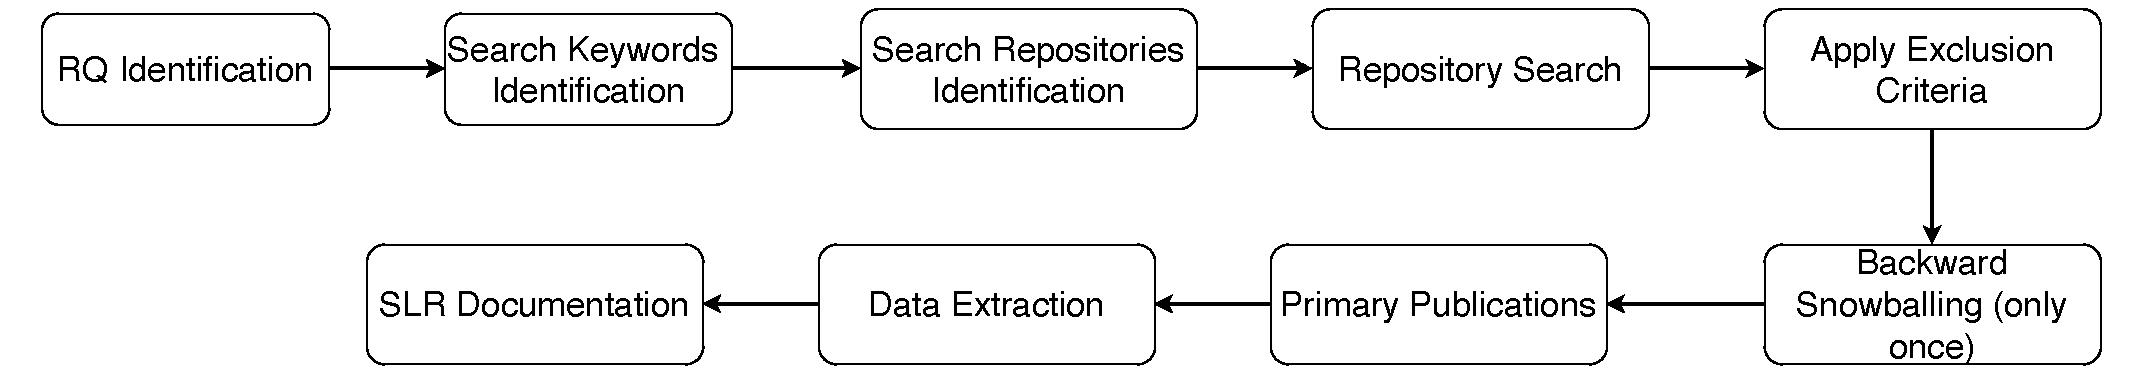
\includegraphics[width=1\linewidth]{figures/SLR.drawio.pdf}
    \caption{An overview of the systematic literature review process.}
    \label{fig:slr-overview}
\end{figure}

\subsubsection{Search Datasets}
We used four well-known repositories, namely ACM Digital Library \footnote[1]{http://dl.acm.org/}, IEEE Xplore Digital Library \footnote[2]{http://ieeexplore.ieee.org/}, Springer Link \footnote[3]{http://link.springer.com/}, and Google Scholar \footnote[4]{https://scholar.google.com/}. Some of these repositories impose restrictions on the amount of search result metadata that can be downloaded. For instance, Google Scholar does not allow frequent search requests from a single device via its API. To overcome this limitation, we used Publish or Perish \footnote[5]{https://harzing.com/resources/publish-or-perish}, a tool that helps retrieve academic documents from Google Scholar. Similarly, Springer Link limits metadata downloads to the first 1,000 search results. However, our search query yielded approximately 10,000 results on this repository. Manually downloading metadata in batches would have been tedious and time-consuming. To handle this efficiently, we used Python scripts to extract data from Springer Link, IEEE Xplore, and ACM Digital Library.

\subsubsection{Exclusion Criteria}
The search terms we used were quite broad, resulting in an exhaustive list of publications. Due to this broad scope, many papers in the search results may be irrelevant to our review. To refine our selection and exclude non-relevant papers, we applied specific exclusion criteria, which are detailed below:

\begin{enumerate}
    \item Given that the majority of scientific publications today are in English, we exclude all non-English papers from our review.
    \item Papers under 5 pages in double-column format or under 7 pages in LNCS single-column format were excluded. Additionally, papers exceeding 30 pages in LNCS single-column format were also excluded.
    \item If multiple papers described the same or similar approaches, we included only the one with the most comprehensive description. For example, an extended journal paper \cite{lu2021eagle} was selected over its shorter conference version \cite{lu2020precision}.
    \item Papers lacking sufficient technical details about their approaches were excluded.
    \item Papers that did not focus on optimizing static analysis itself were excluded. For example, papers that use static analysis to optimize the analyzed program were considered out of scope and excluded.
    \item Papers that focus on dynamic or hybrid analysis were excluded.
\end{enumerate}


\subsubsection{Primary publications selection}
Table \ref{tab:summary_slr} summarizes the results of the search process. For each paper, we first reviewed the title and keywords to determine its relevance to our use case. If the relevance was unclear, we proceeded to read the abstract. If the abstract was still insufficient to make a decision, we skimmed the paper to assess its suitability.
\todo{Usually here we should discuss how many reviewers did read the paper, and how did you overcome the inconsistencies the results?}
In the end, we got \noofpapers papers in total.

\subsubsection{Backward snowballing}
To ensure the completeness of our study and to capture relevant works not identified through our initial search terms, we conducted a lightweight backward snowballing process, performed only once.
The objective was to identify additional papers cited by our initially selected primary publications that align with the scope of our study.
Manual snowballing process it tedious and time consuming, so we developed a series of python scripts to automate and streamline the process.
First, We used pdfx \footnote{https://github.com/metachris/pdfx} to extract the text from the pdf and then retrieved the references from the extracted text.
Subsequently, additional scripts were used to filter out papers which fell outside the defined year boundary of our study scope.
Furthermore, we used python scripts to extract keywords from the paper, and eliminated those that did not align with the scope of our review.
After the automatic filtering stage, we manually reviewed the titles and abstracts of the remaining references. 
Papers found relevant to the scope of study, and not already included in our primary publications set were added to the final list of primary publications.
The relatively high number of additional papers identified through backward snowballing can be attributed to the fine-grained terms used by the original studies, which were not fully covered by our broader search strategy.
For instance, many papers contains keywords such as context-sensitivity, context, parallel processing, call graph, call site sensitivity, which, although highly relevant, were not explicitly included in our original search queries.
Our initial search term aimed for broader coverage, while snowballing allowed us to capture these more granular studies.


\begin{table}
    \begin{tabular}{lccccc}
    \toprule
    Source                         & IEEE & ACM  & Springer & Google Scholar & Total \\
    \midrule
    Search Results                 & 5561 & 3195 & 3980     & 1000           & 13736 \\
    After Reviewing Title/Keywords & 44   & 136  & 13       & 43             & 317   \\
    After Reading Abstracts        & 117  & 30   & 22       & 2              & 171   \\
    After Skimming                 & 72   & 22   & 3        & 20             & 117   \\
    After Final Discussion         &      &      &          &                & 96    \\
    Backward snowballing           &      &      &          &                & 28    \\
    Total                          &      &      &          &                & 124    \\ 
    \bottomrule
    \end{tabular}
    \caption{Summary of the Primary Publications Selection Process}
    \label{tab:summary_slr}
\end{table}
    
\section{Graphs}
Understanding how control flows through the program, how data moves between the variables, and how different program components
depend on each other is a very crucial thing to know before any analysis.

There are 4 different widely used graph structures for them namely Control Flow Graph (CFG), Value Flow Graph (VFG), Program Dependence Graph (PDG), and System Dependence Graph (SDG)

Graphs

- Flow-sensitive, context-sensitive, and object-sensitive information flow control based on program dependence graphs (Hammer et al., 2009):
The Information Flow Control (IFC) is used to analyze a program for security leaks. Existing approaches are not precise enough, that means they report too many false alarms. Therefore in this paper 
they use program dependence graphs (PDG) for Java bytecode to implement IFC. Their approach is more precise and it is flow-, context and object-sensitive. One limit of their approach is that 
they can only deal with medium-sized programs (up to 100kLOC).

-  Speeding up context-, object- and field-sensitive SDG generation (Graf, 2010):  In their presented approach they generate SDGs (System dependence graph) efficiently for Java. It is context-, 
field- and object-sensitive and is based on the WALA framework. They showed that their approach reduces time and memory and can improve precision. The technqical background is that the size of object trees 
can become large if the points-to analysis is less precise, so they can't be used in SDGs. In their paper they introduce object graphs, an extension of object tress. As a result they merge duplicate information 
to save space. 

-  Quantitative Interprocedural Analysis (Chatterjee et al., 2015):  They present an efficient algorithm which can answer several static analysis questions, e.g. estimating the average energy consumption (cite).
For that they need the ICFG and a positive weight function which determines for every transition a positive number which says how good, bad or neutral this transition (event) is. 
After that their algorithm compares the good and bad events and determine whether a given threshold is reached in a run. As a result they can quantify the ICFG. Their algorithm is implemented in the Java soot framework 
and can deal with recursion and is sound. But one limit is that they have not consider mulitple quantitative objectives yet but are aiming that in the future. (TODO: have they already done that and can we find improvements?)

-  A Precise Framework for Source-Level Control-Flow Analysis (Riouak et al., 2021):  Their presented framework is called INTRACFG which constructs precise intraprocedrual CFGs. It is based on reference 
attribute grammers and enables the construction of CFGs which are independent of the shape and structure of the AST because other frameworks for constructing CFGs are usually depending from the structure of ASTs. 
INTRACFG only connects AST nodes of interest in the CFG. Attribute grammers denote AST nodes with attributes, reference attribute grammers extend them: their values are references to other AST nodes (cite). 
In their work they achieved to reduce the number of nodes and edges in the CFGs by over 30% compares to other framework. 

-  Efficient Path-Sensitive Data-Dependence Analysis (Yao et al., 2021):  They present a path- and context-sensitive data-dependence analysis with the goal to solve the  aliasing-path-explosion problem 
via a sparse and demand-driven approach. The exisiting challenge for data-dependence analysis is the aliasing-path-explosion problem which means to tracks a large amount of aliases. Their approach summarizes 
data dependence as symbolic and storeless value-flow graphs and they perform a demand-driven phase that resolves transitive data dependence over the graphs. The presented framework is called FALCON, a fused and 
sparse approach for path-sensitive data-dependence analysis. First their approach computes storeless value-flow graphs, as a result no duplicated edges. Then this graph is used for data-dependencies in a 
demand-driven way. By that a path- and context-sensitive def-use information is tracked on demand. It is more efficient because the data dependency can be figured out without points-to information 

-  Path-Sensitive Sparse Analysis without Path Conditions (Shi et al., 2021) :  The sparse program analysis considers only necessary control flows but is still expensive for path-sensitive analysis (cite). 
In this work the authors present Fusion, a fused approach to inter-procedurally path-sensitive sparse analysis (cite). They can determine the path feasiblity without knowing the path conditions, 
this saves cost and time. In their approach the SMT solver works on the program data dependece graph. That's how they can determine path feasibility directly.
They showed that they were able to detect a lot of bugs in mature open-source software with their approach,faster than two other state-of-art approaches. Fusion can analyze milliones of lines of code within a 
short time and less memory compared to other approaches. They achieved the precision of inter-procedural path-sensitivity.


\bibliographystyle{ACM-Reference-Format}
\bibliography{bibliography}

\end{document}
\endinput
